\section{700 --- Search in a Binary Search Tree}

\textbf{Easy}

Given the root node of a binary search tree (BST) and a value. You need to find the node in the BST that the node's value equals the given value. Return the subtree rooted with that node. If such node doesn't exist, you should return \fcc{NULL}.

For example, 

Given the tree:

\begin{figure}[H]
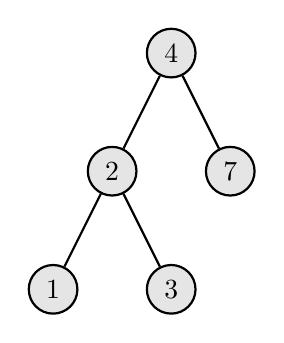
\begin{tikzpicture}
[every node/.style={draw, circle, fill=gray!20!, minimum size=5mm},
thick]
\node{4}
child{node{2} child{node{1}} child{node{3}}}
child{node{7}};
\end{tikzpicture}
\end{figure}
%        4
%       / \
%      2   7
%     / \
%    1   3

And the value to search: 2

You should return this subtree:

\begin{figure}[H]
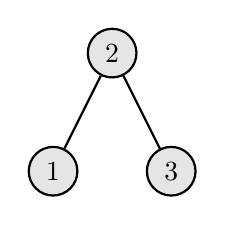
\begin{tikzpicture}
[every node/.style={draw, circle, fill=gray!20!, minimum size=5mm},
thick]
\node{2}
child{node{1}}
child{node{3}};
\end{tikzpicture}
\end{figure}
%
%      2     
%     / \   
%    1   3
In the example above, if we want to search the value 5, since there is no node with value 5, we should return \fcc{NULL}.

Note that an empty tree is represented by \fcc{NULL}, therefore you would see the expected output (serialized tree format) as \fcc{[]}, not \fcj{null}.

\subsection{BST Search}
Typical BST Search Problem

\setcounter{lstlisting}{0}
\begin{lstlisting}[style=customc, caption={BST}]
TreeNode* searchBST( TreeNode* root, int val )
{
    if( !root )
    {
        return nullptr;
    }
    auto t = root;
    while( t )
    {
        if( t->val == val )
        {
            return t;
        }

        if( t->val < val )
        {
            t = t->right;
        }
        else
        {
            t = t->left;
        }
    }
    return t;
}
\end{lstlisting}